\subsubsection{Energy Consumption Model for Nano Data Centers}

While nano data centers are motivated by the energy consumption problem~\cite{DBLP:conf/conext/ValanciusLMDR09},
current research reveals that the advantage of the nano data centers in energy efficiency relies on certain technical foundations.
To give an overview of the technical challenges towards nano data center development,
we first need to figure out the energy consumers of the nano data center applications.

Considering the nano data center (NaDa) platform proposed in~\cite{DBLP:conf/conext/ValanciusLMDR09},
users will host tiny managed nano servers on their end-user devices such as Triple-Play gateways and DSL/cable modems,
and communicate with each other following a Peer-to-Peer (P2P) philosophy.
Thus, suppose a user (client) wants to access the content stored in a nano server hosted by another user (manager),
the energy consumption for this process consists of~\cite{DBLP:journals/sigmetrics/JalaliAVHAT14}:
\begin{itemize}
\item the energy consumed by the client for requesting the content, denoted as $E_\text{req}$;
\item the energy consumption of the content transportation process, denoted as $E_\text{trans}$; and
\item the energy consumed by the manager for storing the content and processing the request, denoted as $E_\text{serv}$.
\end{itemize}
If we denote the total energy consumption as $E_\text{total}$, we can derive the following formula:
\begin{equation}
E_\text{total}=E_\text{req}+E_\text{trans}+E_\text{serv} \label{abstract_model}.
\end{equation}

To detail the formula from technical aspects, we need to understand the internet protocol (IP) network.
\cite{iptv} modeled the IP network as the combination of three domains:
the access network, the metropolitan and edge networks and the core network.
For centralized data center applications,
\cite{iptv} visualized the IP network model as shown in Figure~\ref{fig:ipnet}.
The access network connects each end-user to the metropolitan and edge network,
which serves as the interfaces to the core network.
Centralized data centers are usually directly connected with the core network,
but for nano data centers, since nano servers are hosted in end-user devices,
the data has to traverse the access network twice~\cite{tradeoff}.
 
\begin{figure}[h]
	\fontsize{12}{12} \selectfont
	\centerline{\resizebox{15cm}{!}{\input{image/IPnetwork.eps_tex}}}
	\caption{IPTV network model for centralized data centers~\cite{iptv}}
	\label{fig:ipnet}
	\normalsize
\end{figure}

We can now detail formula (\ref{abstract_model}) and adapt it to the energy consumption model proposed in~\cite{DBLP:journals/sigmetrics/JalaliAVHAT14} as the following:
\begin{align}
E_\text{req}&=E_{c}+E_\text{access},\\
E_\text{trans}&=E_\text{edge}\cdot h_\text{edge}+E_\text{core}\cdot h_\text{core},\\
E_\text{serv}&=E_\text{access}+ E_{m},
\end{align} 
where $E_c$ represents the energy consumed in the end-user device of the client, 
$E_\text{access}, E_\text{edge}$, and $E_\text{core}$ represent the energy consumed in the access network, edge network and core network, respectively, 
$h_\text{edge}$ and $h_\text{core}$ represent the number of hops in the edge and core networks,
and $E_m$ represents the energy consumed in the end-user device of the manager.

In the following, we will introduce four technical challenges that we regard as fundamental and argument our selections with respect to the proposed energy consumption model.
These challenges are:
the activation of nano servers;
the selection of the access network that the nano servers are attached to; 
the location of nano servers;
and the number of data replication strategy.

\subsubsection{Activation of Nano Servers}

A nano data center platform is constructed with end-user devices as nano servers.
We refer a nano server as \textit{active}, when it is on and the user is accessing the nano data center service,
and we refer a nano server as \textit{idle}, when it is on but the user is not accessing the nano data center service.
Whenever a nano server is on,
no matters it is active or idle,
it consumes energy.
\cite{DBLP:conf/conext/ValanciusLMDR09} proposed a thorough study on how the activation status of nano servers affects the total energy consumption.
\cite{DBLP:conf/conext/ValanciusLMDR09} denoted the active times of a nano server as $t_\text{act}$ and the idle time of the nano server as $t_\text{idle}$,
and introduced a coefficient $R$ that represents the ratio of the active time of nano servers to the whole duration when nano servers are on:
\begin{equation}
R=\frac{t_\text{act}}{t_\text{act}+t_\text{idle}}.\\
\end{equation}
As proposed in~\cite{DBLP:conf/conext/ValanciusLMDR09}, 
$R$ is involved in the calculation of both $E_c$ and $E_m$ in the energy consumption model.
As a result,
the energy consumption of nano data centers correlates with $R$ as shown in Figure~\ref{fig:active},
where five different active time ratios (0.01, 0.05, 0.2, 0.5, 1) are chosen for comparison,	
and the energy consumption of a centralized data center is also shown as a reference.
We can see that the energy consumption of nano servers increases as the active time ratio decreases,
and when the ratio is large than 0.2, the energy consumption of nano servers surpasses the energy consumption of the centralized data center,
i.e. the nano data center becomes less energy efficient.

\begin{figure}[h]
	\fontsize{12}{12} \selectfont
	\centerline{\resizebox{5cm}{!}{\input{image/chart2.eps_tex}}}
	\caption{Energy consumption of nano servers with different active time ratio, and of a centralized data center~\cite{DBLP:conf/conext/ValanciusLMDR09}}.
	\label{fig:active}
	\normalsize
\end{figure}

A disappointing fact is that we cannot simply assume the active time ratio $R$ to be higher than $0.2$ most of the time.
Taking the widely-used video delivered by Internet protocol (IPTV)  as an example:
according to~\cite{DBLP:conf/conext/ValanciusLMDR09} and~\cite{watchingTV},
the IPTV user activity shows large variation throughout the day,
as shown in Figure~\ref{fig:iptv}.
Even the in the peak hour,
fewer than $20\%$ of customers are active (i.e. $R<0.2$);
as for in the midnight,
less than $5\%$ of customers are active (i.e. $R<0.05$).
On average,
the active ratio $R$ is around $0.07$,
which means that if all nano servers are on in the whole day,
it is energy \textbf{in}efficient to apply nano data centers.

\begin{figure}[h]
	\fontsize{12}{12} \selectfont
	\centerline{\resizebox{5cm}{!}{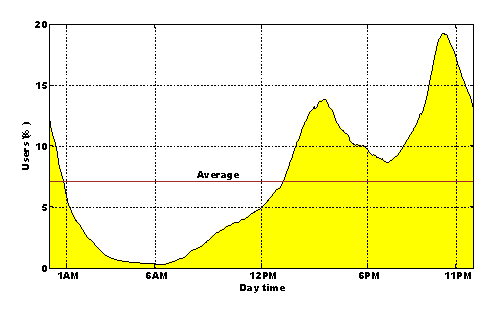
\includegraphics{image/chart3.eps}}}
	\caption{User activity of the IPTV service~\cite{DBLP:conf/conext/ValanciusLMDR09}}.
	\label{fig:iptv}
	\normalsize
\end{figure}

Therefore, to make a nano data center platform energy-efficient,
it is necessary to increase the active time ratio.
From our view,
a possible solution is to turn off the nano server time to time to reduce the idle time of the nano servers.
But for the nano servers attached to DSL-modems or other functional devices,
such as the NaDa model proposed in~\cite{DBLP:conf/conext/ValanciusLMDR09},
turning off nano servers can lead to side-effects on the usage of other internet services of users,
and thus the implementation of this solution requires further study.
Another possible solution is to modify the applications for the nano data center,
such as run multiple applications that have different peak hours,
aiming to maximize the active time of the nano servers.
So far we are unaware of any research tackling these problems,
and thus we list the activation of nano servers as one of the four technical challenges towards nano data center development.

\subsubsection{Access Network}

\subsubsection{Location of Nano Servers}

\subsubsection{Data Replication}
